\documentclass{article}

\title{Metodi Numerici per l'Informatica}
\author{Anthony}
\date{7 mar 2023}

\usepackage{amssymb}
\usepackage{amsmath}
\usepackage{xcolor}
\usepackage{cancel}
\usepackage{graphicx}
\usepackage[font=small,labelfont=bf]{caption}

\newcommand*{\horzbar}{\rule[.5ex]{2.5ex}{0.5pt}}

\begin{document}
    \maketitle
    \section{Regressione lineare -- introduzione}
        Consideriamo il seguente problema di fitting: dato un insieme di punti in $\mathbb{R}^2$, vogliamo estrarre un'equazione 
        che \emph{fitta} quei punti.
        \begin{center}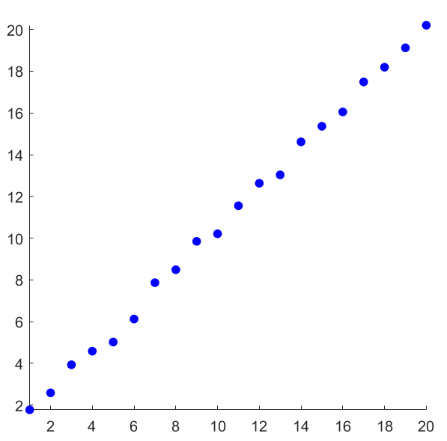
\includegraphics[width=5.3cm]{graph_01.png}\end{center}
        In questo caso è una retta. Dato l'insieme di $x$, vogliamo trovare i coefficienti $a, b$ tali che riescano a soddisfare la 
        seguente equazione lineare:
        \[y = ax + b\]
        \begin{center}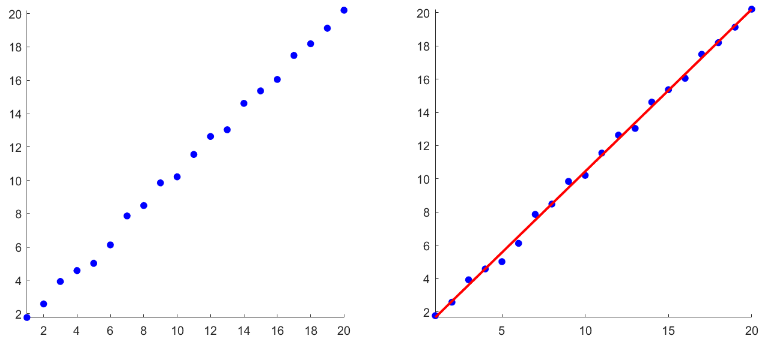
\includegraphics[height=4.71cm]{graph_02.png} \end{center}
        Questo è un problema di \emph{regressione}: abbiamo i dati e vogliamo estrarre i parametri. Abbiamo ora scelto un \emph{modello},
        ovvero un'equazione lineare più un certo bias. I parametri da trovare sono $\Theta = {a,b}$.
            \[f_\Theta(x_i) = y_i \]
        L'equazione $f_\Theta(x_i) = y_i$ deve valere per $i=1, \dots, n$. I vari punti $x_i$ sono chiamati \emph{regressori}, poiché stiamo risolvendo un problema di regressione.

        \subsection{Errore quadratico medio}
            Per trovare i coefficienti $a,b$ abbiamo bisogno di un nuovo formalismo: il formalismo dell'\emph{ottimizzazione numerica}.
             Siamo di fronte a un problema di minimizzazione; In questo caso vogliamo trovare $a,b$ tali che minimizzano l'errore 
             quadratico medio, anche detto MSE, tra input e l'output previsto.
                \[ \epsilon = \min_{a,b \in \mathbb{R}} \frac{1}{n} \sum_{i=1}^{n}(y_i - f_\Theta(x_i))^2 \]
            Vogliamo trovare i valori di $a,b$ per cui la differenza tra i punti $x_i$ e i valori generati da una certa \emph{funzione obiettivo} 
            $f$ sia più piccola possibile.
            I \emph{minimizzatori} sono l'argomento $\Theta$, che minimizza $f$. Vogliamo un algoritmo che, dato un problema di regressione, 
            ci trovi i minimizzatori. \\
            Questo è chiamato il \emph{problema di approssimazione dei minimi quadrati}, o least-squares approximation; c'è l'errore 
            quadratico medio, $f$ è lineare più un certo bias. Per risolvere questo problema di ottimizzazione ci servono altri due 
            concetti: \emph{convessità} e \emph{gradiente}.

            \paragraph{Ottimizzazione}
                Abbiamo quindi osservato che siamo di fronte a un problema di \emph{minimizzazione}. La forma generale per risolvere un problema
                di questo tipo è la seguente:
                    \[\epsilon = \min_x f(x)\]
                Risolvere un problema del genere richiede quindi di trovare:
                \begin{enumerate}
                    \item Un minimizzatore $\mathbf{x^*} = \arg \min_\mathbf{x}f(\mathbf{x})$
                    \item Un minimo $\epsilon = f(\mathbf{x^*})$
                \end{enumerate}
    
        \subsection{Convessità}
            Intuitivamente, dati due punti che passano per una funzione, se la retta che passa tra i due punti è sempre sopra la funzione,
            allora la funzione è \emph{convessa}. Più formalmente, questo è dimostrabile attraverso la \emph{disuguaglianza di Jensen}:
            \[ f(\alpha x + (1-\alpha)y) \leq \alpha f(x) + (1-\alpha)f(y) \text{ }\forall x,y \text{ e }\alpha \in (0,1)\]
            \begin{center}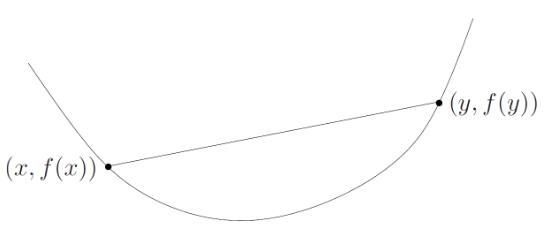
\includegraphics[width=10cm]{jensen.png}\end{center}
            \captionof{figure}{Disuguaglianza di Jensen}
            Assumiamo che $f$ sia differenziabile, così possiamo computare la sua derivata $\frac{df}{dx}$ in ogni punto $x$. Intuitivamente, possiamo 
            dire che i minimizzatori di una funzione convessa hanno la derivata pari a zero; cerchiamo il minimizzatore $x$ tale che 
            $\frac{df(x)}{dx}=0$.

            \subsubsection{Funzioni convesse: minimo globale}
                Per trovare il minimo globale, partiamo dalla definizione di convessità:
                \[f(\alpha x + (1-\alpha)y) \leq \alpha f(x) + (1-\alpha)f(y) =\]
                \[f(x + \alpha(y-x)) \leq (1-\alpha)f(x) + \alpha f(y) =\]
                \[\frac{f(x + \alpha(y-x))}{\alpha} \leq \frac{(1-\alpha)f(x) + \alpha f(y)}{\alpha}\]
                \[\frac{f(x + \alpha(y-x))}{\alpha} \leq \frac{f(x)}{\alpha} - f(x) + f(y)\]
                \[\frac{f(x + \alpha(y-x)) - f(x)}{\alpha}+f(x) \leq f(y)\]
                \[\lim_{\alpha \to 0} \frac{f(x + \alpha(y-x)) - f(x)}{\alpha}+f(x) \leq f(y)\]
                \[\lim_{\alpha \to 0} \frac{f(x + \alpha(y-x)) - f(x)}{\alpha}(y-x)+f(x) \leq f(y)\]
                \[\frac{df(x)}{dx}(y-x) + f(x) \leq f(y)\]

                Abbiamo ottenuto una serie di Taylor del primo ordine.
                \begin{center}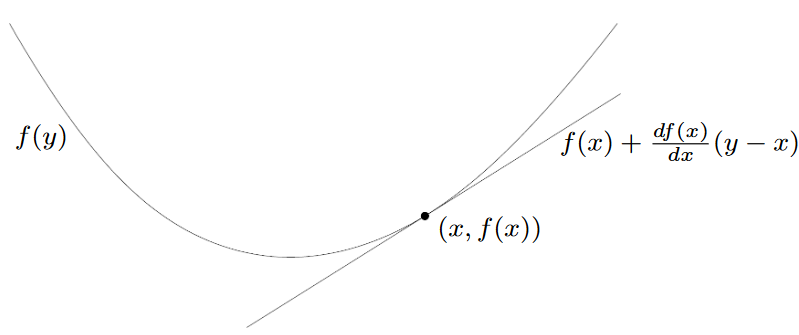
\includegraphics[width=9.2cm]{taylor.png}\end{center}
                Per cui, se $\frac{df(x)}{dx}=0$:
                \[f(x) \leq f(y)\]
                Risolvendo per $x$ significa che trovare un minimo globale.
            \subsection{Funzioni convesse: conclusioni}
                Se $f(x)$ è convessa, allora è possibile trovare il suo minimo globale settando la sua derivata a zero
                $\frac{df(x)}{dx}=0$ e risolvendo per $x$. Questo ha ovviamente senso solo se $f : \mathbb{R} \to \mathbb{R}$.
                Se $f(\mathbf{x})$ è multi-dimensionale, ad esempio $f: \mathbb{R}^n \to \mathbb{R}$, dobbiamo estendere i concetti di 
                convessità e derivata a funzioni multi-dimensionali.

    \section{Il gradiente}
        In generale, avremo a che fare con funzioni con $n \gg 1$ variabili:
                \[f:\mathbb{R}^n \to \mathbb{R}\]
        In questi casi, la nozione di derivata è rimpiazzata dal \emph{gradiente}:
                \[\nabla_\mathbf{x}f(x) = \begin{pmatrix}
                    \frac{\partial f}{\partial x_1} \\
                    \vdots \\
                    \frac{\partial f}{\partial x_n}
                \end{pmatrix} \]
        Il gradiente non è altro il vettore delle derivate parziali di $f$ difatti, data una semplice funzione con dominio uni-dimensionale, 
        la nozione di derivata è equivalente a quella del gradiente.\\
        La convessità è invece definita come prima. Cambia solo il dominio in cui sono definiti $\mathbf{x}$ e $\mathbf{y}$:
        \[f(\alpha \mathbf{x} + (1-\alpha)\mathbf{y}) \leq \alpha f(\mathbf{x}) + (1-\alpha)f(\mathbf{y}) =\]
        Come il piano cartesiano, rimane invariata la condizione di ottimalità:
        \[\nabla_\mathbf{x} f(\mathbf{x}) = \mathbf{0} \implies f(\mathbf{x}) \leq f(\mathbf{y}) \text{ }\forall \mathbf{y} \in \mathbb{R}^n\]
        
        \newpage

        Il gradiente $\nabla_\mathbf{x}f(\mathbf{x})$ codifica la direzione verso cui vi è la \emph{maggior crescita} di $f$ rispetto a un punto 
        $\mathbf{x}$. Ad esempio, in un caso 1-dimensionale:
        \begin{center}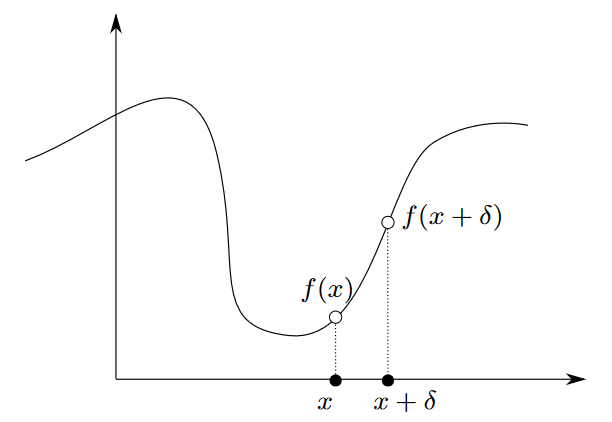
\includegraphics[width=10cm]{gradient.png}\end{center}

        Il gradiente vive nel dominio della funzione ed è bene interpretarlo come un \emph{campo di freccette} definito sul dominio.
        \begin{center}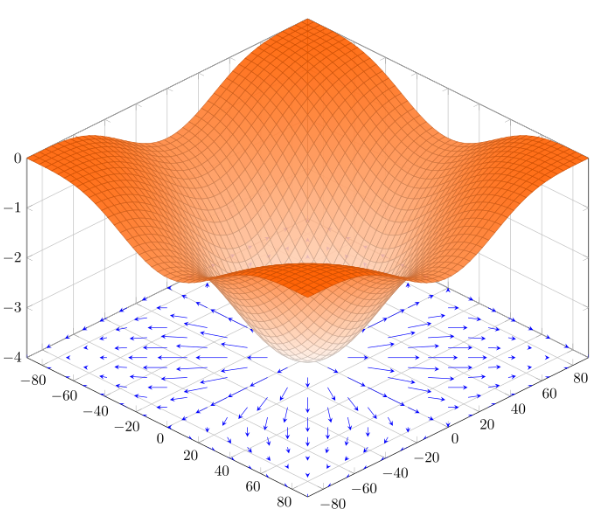
\includegraphics[width=10cm]{gradient_2.png}\end{center}
        La lunghezza del vettore codifica la ripidità della funzione, e le derivate codificano esattamente come è fatta la funzione; 
        difatti è possibile integrare il campo del gradiente e riottenere la funzione da cui siamo partiti.

        \subsection{Lunghezza dei vettori}
            Il nostro scopo è quello di misurare la lunghezza del gradiente. In $\mathbb{R}^2$ possiamo applicare il teorema di 
            Pitagora per capire quanto sono distanti due punti. Il teorema di Pitagora è anche chiamato, nel caso più generale, distanza Euclidea:
            \begin{center}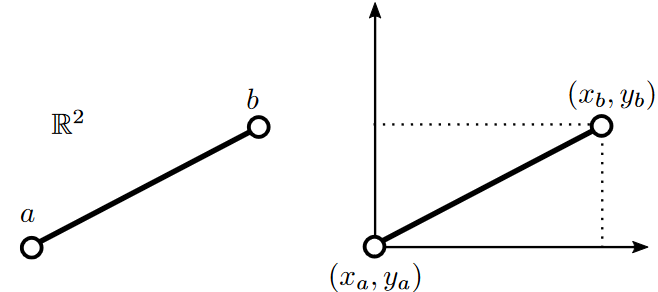
\includegraphics[width=10cm]{euclidean_distance.png}\end{center}
            Da cui otteniamo:
            \[d(a,b) = (|x_b - x_a|^2 + |y_b - y_a|^2)^{\frac{1}{2}}\]
            Il teorema di Pitagora, in nozione matriciale, può anche esser scritto nel seguente modo:
                \[d(\mathbf{a},\mathbf{b}) = \Vert \mathbf{a} - \mathbf{b} \Vert_2\]
            In cui $\mathbf{a} = \begin{pmatrix}
                x_a \\
                y_a
            \end{pmatrix}$ e $\mathbf{b} = \begin{pmatrix}
                x_b \\
                y_b
            \end{pmatrix}$ \\

            Da questa definizione di distanza, possiamo calcolare la lunghezza di un vettore $\mathbf{x}$ come la distanza dall'origine a 
            $\mathbf{x}$:
                \[\Vert \mathbf{x} - \mathbf{0} \Vert_2 = \Vert \mathbf{x} \Vert_2 = \sqrt{\mathbf{x}^T\mathbf{x}} \]
            Questa distanza si chiama \emph{norma}. 
            Spesso, per semplicità e per evitare di computare le radici quadrate, consideriamo il quadrato della norma:
                \[\Vert \mathbf{x} \Vert_2^2 = \mathbf{x}^T\mathbf{x}\]

    \section{La soluzione della regressione lineare}
        Il nostro scopo è, come abbiamo già osservato, trovare gli $a,b$ che minimizzano l'espressione:
            \[\mathbf{\Theta}^* = \arg \min_{\mathbf{\Theta} \in \mathbb{R}^2} \ell(\mathbf{\Theta})\]
        In cui $\ell:\mathbb{R}^2 \to \mathbb{R}$ definita come segue:
            \[\ell(a,b) = \sum_{i=1}^n (y_i - ax_i - b)^2 \]
        Abbiamo una soluzione settando il gradiente a zero, ovvero  $\nabla_{\mathbf{\Theta}} \ell(\mathbf{\Theta}) = \mathbf{0}$.
        Per la linearità del gradiente, e in particolare poiché il gradiente gode dell'additività, possiamo scrivere:
            \[\nabla_{\mathbf{\Theta}}\sum_{i=1}^n (y_i - ax_i - b)^2 = \sum_{i=1}^n \nabla_{\mathbf{\Theta}} (y_i - ax_i - b)^2\]
        Possiamo osservare che $y_i$ è costante rispetto ad $a,b$, quindi possiamo eliminarlo. Espandiamo anche il quadrato:
            \[= \sum_{i=1}^n \nabla_{\mathbf{\Theta}} (\cancel{y_i^2} + a^2x^2_i + b^2 - 2x_iy_i - 2by_i + 2abx_i) \]
        E per le proprietà della sommatoria otteniamo la seguente espressione:
            \begin{equation} 
                = \begin{pmatrix} \sum_{i=1}^n 2ax_i^2 - 2x_iy_i + 2bx_i \\
                \sum_{i=1}^n 2b - 2y_i + 2ax_i \end{pmatrix}
            \end{equation}
        Otteniamo quindi due equazioni lineari nelle incognite $a,b$ da settare a zero:
        \begin{equation} 
            = \begin{pmatrix} \sum_{i=1}^n 2ax_i^2 - 2x_iy_i + 2bx_i \\
            \sum_{i=1}^n 2b - 2y_i + 2ax_i \end{pmatrix} 
            = \begin{pmatrix}
                0 \\
                0
            \end{pmatrix}
        \end{equation}
        In questo modo abbiamo risolto il problema di minimizzazione.
    \section{Regressione lineare: notazione matriciale}
        Quando usiamo metodi numerici, manipoliamo matrici e vettori per cui vogliamo esprimere la regressione lineare con la notazione 
        matriciale:
        \[ \underbrace{\begin{pmatrix}
            y_1 \\
            y_2 \\
            \vdots \\
            y_n
        \end{pmatrix}}_\mathbf{y} = \underbrace{\begin{pmatrix}
            x_1 & 1 \\
            x_2 & 1 \\
            \vdots & \vdots \\
            x_n & 1 \\
        \end{pmatrix}}_\mathbf{X} \underbrace{\begin{pmatrix}
            a \\
            b
        \end{pmatrix}}_\mathbf{\theta}\]
    Tale notazione esprime tutte le equazioni della forma $y_i = ax_i + b$ e fa sì che la linearità rispetto a $a,b$ sia evidente. L'errore
    quadratico medio, espresso con la norma Euclidea, è semplicemente:
        \[ \ell(\mathbf{\theta}) = (\mathbf{y} - \mathbf{X\theta})^T (\mathbf{y} - \mathbf{X\theta}) \]
        \[ = \mathbf{y}^T \mathbf{y} - 2\mathbf{y}^T\mathbf{X\theta} + \mathbf{\theta}^T \mathbf{X}^T\mathbf{X\theta} \]
        E settando il gradiente, ovvero le derivate rispetto a $\theta$, uguale a zero otteniamo:
        \[ -2\mathbf{X}^T\mathbf{y} + 2\mathbf{X}^T\mathbf{X\theta} = \mathbf{0} \]
        \[ = \mathbf{X}^T\mathbf{X\theta} = \mathbf{X}^T\mathbf{y}\]
        E possiamo risolvere tale equazione per $\theta$ risolvendo il sistema lineare:
        \[\mathbf{\theta} = (\mathbf{X}^T\mathbf{X})^{-1}\mathbf{X}^T\mathbf{y}\]

        Con ciò abbiamo ottenuto una \emph{forma chiusa} del nostro problema iniziale.
    \section{Regressione lineare: grandi dimensioni}
        Abbiamo risolto i casi in cui $x,y$ sono semplici numeri, ma anche se scaliamo a più dimensioni otteniamo una simile soluzione.
        In generale, siano $(\mathbf{x}_i, \mathbf{y}_i)$ vettori in $\mathbb{R}^d$:
            \[\mathbf{y}_i = \mathbf{Ax}_i + \mathbf{b} \quad \forall i=1,\dots,n\]
        Accorpando tutti i data points nella matrice $\tilde{\mathbf{X}} = \begin{pmatrix}
            \vline       & \vline       & \\
            \mathbf{x}_1 & \mathbf{x}_2 & \dots \\
            \vline       & \vline       & 
        \end{pmatrix}$ e $\mathbf{Y}$ otteniamo:
        \[\underbrace{\begin{pmatrix}
            y_{11} & \dots & y_{1d} \\
            y_{21} & \dots & y_{2d} \\
            \vdots &       & \vdots \\
            y_{n1} & \dots & y_{nd} \\
        \end{pmatrix}}_{\mathbf{Y}^T} = \underbrace{\begin{pmatrix}
            x_{11} & \dots & x_{1d} & 1\\
            x_{21} & \dots & x_{2d} & 1\\
            \vdots &       & \vdots & 1\\
            x_{n1} & \dots & x_{nd} & 1\\
        \end{pmatrix}}_{\mathbf{X}^T := (\tilde{\mathbf{X}}^T | 1)}
        \underbrace{\begin{pmatrix}
            a_{11} &  \dots & a_{1d} \\
            \vdots &        & \vdots \\
            a_{d1} &  \dots & a_{dd} \\
            b_1    &  \dots & b_d 
        \end{pmatrix}}_\mathbf{\Theta}
        \]
        Per cui, per ogni data point $\mathbf{y}_i$ otteniamo:
        \[
            \begin{pmatrix}
                y_{i1} \\
                \vdots \\
                y_{id}
            \end{pmatrix} =
            \begin{pmatrix}
                \sum_{j=1}^d a_{j1}x_{ij} + b_1 \\
                \vdots \\
                \sum_{j=1}^d a_{jd}x_{ij} + b_d
            \end{pmatrix}
        \]
        L'errore quadratico medio è quindi:
        \[\ell(\Theta) = \Vert \mathbf{Y}^T - \mathbf{X}^T \mathbf{\Theta} \Vert_2^2 = tr(\mathbf{Y}^T\mathbf{Y}) - 2tr(\mathbf{YX}^T\mathbf{\Theta}) + tr(\mathbf{\Theta}^T \mathbf{XX}^T \mathbf{\Theta}) \]
        La formula chiusa della soluzione di $\nabla_\mathbf{\Theta}\ell(\mathbf{\Theta}) = \mathbf{0}$ è:
        \[\mathbf{\Theta} = (\mathbf{XX}^T)^{-1}\mathbf{XY}^T\]

    \section{Regressione polinomiale}
        Finora abbiamo osservato come comportarci in un contesto in cui i punti sono disposti linearmente, ora osserveremo come applicare 
        la regressione polinomiale, a prescindere dell'ordine del polinomio.
        \begin{center}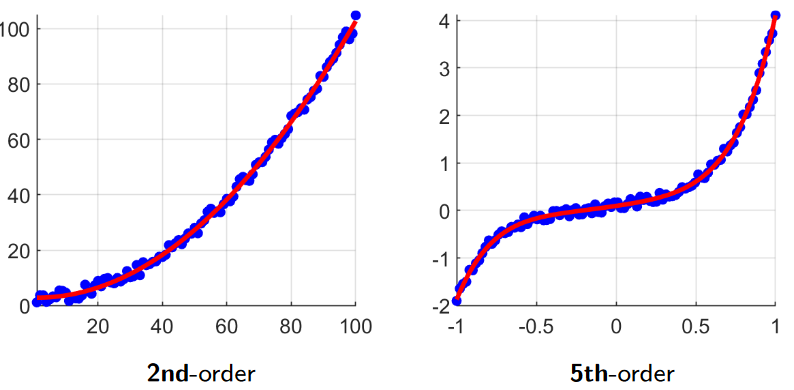
\includegraphics[width=9.8cm]{pol_regr.png}\end{center}
        Il numero di parametri, ovvero le incognite, da trovare cresce con l'ordine del polinomio. Nonostante il nome, la 
        \emph{regressione polinomiale} è lineare nei parametri. È polinomiale rispetto ai dati.
            \[y_i = a_3x_i^3 + a_2x^2_i + a_1x_i + b \quad \forall i=1,\dots,n \]
        Possiamo scrivere l'equazione appena mostrata con una sommatoria:
            \[y_i = \textcolor{red}{b} + \sum_{j=1}^k \textcolor{red}{a_j}x_i^j \quad \forall i=1,\dots,n \]
        In cui le incognite sono $b$ e $a_j$. Mostriamo l'equazione in notazione matriciale:
        \[
            \underbrace{\begin{pmatrix}
                y_{1}\\
                y_{2} \\
                \vdots \\
                y_{n} \\
            \end{pmatrix}}_\mathbf{y} = \underbrace{\begin{pmatrix}
                x_1^k & x_1^{k-1} & \dots & x_1 & 1 \\
                x_2^k & x_2^{k-1} & \dots & x_2 & 1 \\
                \vdots & \vdots & \vdots & \vdots & \vdots \\
                x_n^k & x_n^{k-1} & \dots & x_n & 1 \\
            \end{pmatrix}}_\mathbf{X}
            \underbrace{\begin{pmatrix}
               \color{red} a_{k}\\
               \color{red}a_{k-1} \\
               \color{red} \vdots \\
               \color{red}a_1 \\
               \color{red}  b
            \end{pmatrix}}_\mathbf{\color{red}\theta} \]

        Nonostante l'apparente complessità, tutti gli elementi sono composti da dei numeri calcolabili e quindi l'operazione è lineare. 
        La soluzione in forma chiusa è analoga a prima, tuttavia se vogliamo risolvere il problema di regressione polinomiale desideriamo 
        almeno tanti punti quante incognite. Quindi abbiamo come requisito il grado del polinomio $k<n$. 

        \section{Teorema di Stone-Weierstrass}
            Sia $f$ una funzione continua su intervallo $[a,b]$, per ogni $\epsilon > 0$ esiste un polinomio $p$ tale che 
            $|f(x) - p(x)|<\epsilon \text{ } \forall x$. Quindi possiamo sempre provare a fittare una qualsiasi funzione con un polinomio.
            Esempio:
            \begin{center}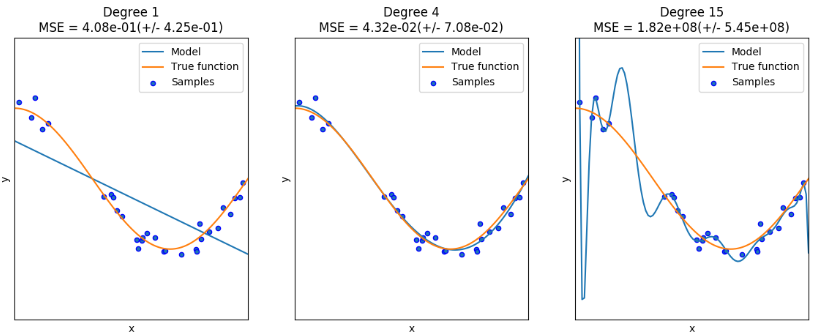
\includegraphics[width=12cm]{stone_weier.png}\end{center}
            A sinistra abbiamo fittato la funzione ignota, disegnata in arancione, con un polinomio di ordine uno e ciò ha generato \emph{underfitting}. La funzione, in particolare,
            cerca di passare mediamente su tutti i punti. Nell'esempio al centro abbiamo invece fittato la funzione con un polinomio di ordine quattro e 
            c'è estrema somiglianza con la funzione ignota. Nell'esempio a destra, infine, abbiamo provato a risolvere il problema 
            di fitting con un polinomio di grado molto alto; esso passa esattamente per tutti i punti ma produce \emph{overfitting}. 
            L'errore del fitting sarà molto basso sui dati attuali, ma la funzione è molto diversa dalla funzione ignota, e quindi la 
            soluzione è errata.
        
        \section{Calcolo del gradiente}
            Abbiamo osservato che l'espressione $y_i = ax_i+b$ può essere espressa in notazione lineare come segue:
            \[ \underbrace{\begin{pmatrix}
                y_1 \\
                y_2 \\
                \vdots \\
                y_n
            \end{pmatrix}}_\mathbf{y} = \underbrace{\begin{pmatrix}
                x_1 & 1 \\
                x_2 & 1 \\
                \vdots & \vdots \\
                x_n & 1 \\
            \end{pmatrix}}_\mathbf{X} \underbrace{\begin{pmatrix}
                a \\
                b
            \end{pmatrix}}_\mathbf{\theta}\]

            Abbiamo anche osservato che l'errore quadratico medio (MSE) è della forma:
            \[\ell(\mathbf{\theta}) = \Vert \mathbf{y} - \mathbf{X\theta} \Vert_2^2 = \mathbf{y}^T\mathbf{y} - 2\mathbf{y}^T\mathbf{X\theta} + \mathbf{\theta}^T\mathbf{X}^T\mathbf{X\theta}\]
            Tale funzione prende in input un vettore e restituisce un numero; possiamo inoltre calcolarne il gradiente, ovvero le derivate parziali
            rispetto a $\theta$; ciò prevede il calcolo di $n$ derivate. Poiché il gradiente è una mappa lineare, possiamo calcolarle
            separatamente. Se settiamo il gradiente rispetto a $\mathbf{\theta}$ a zero otteniamo la seguente espressione:
            \[-2\mathbf{X}^T\mathbf{y} + 2\mathbf{X}^T\mathbf{X\theta} = \mathbf{0}\]
            \paragraph{Esempio} Sia $f(\mathbf{\theta}) = \mathbf{\theta}^T\mathbf{A\theta}$
            \[\nabla_\mathbf{\theta}f(\mathbf{\theta}) = \nabla_\mathbf{\theta}(\mathbf{\theta}_1 \dots \mathbf{\theta}_n) \begin{pmatrix}
                a_{11} & \dots & a_{1n} \\
                \vdots & \ddots &\vdots \\
                a_{n1} & \dots & a_{nn} \\
            \end{pmatrix} \begin{pmatrix}
                \mathbf{\theta}_1 \\
                \vdots \\
                \mathbf{\theta}_n 
            \end{pmatrix}\]

            Osserviamo che tutta l'espressione non è altro che una doppia sommatoria:
            \[\nabla_\mathbf{\theta}f(\mathbf{\theta}) = \nabla_\mathbf{\theta}\sum_{i=1}^n\sum_{j=1}^na_{ij}\mathbf{\theta}_i\mathbf{\theta}_j\]
            Di questa espressione lineare possiamo calcolare tutte le derivate rispetto a ogni $\mathbf{\theta}$:
            \[\nabla_\mathbf{\theta}f(\mathbf{\theta}) = \begin{pmatrix}
                \frac{\partial}{\partial \theta_1}\sum_{i=1}^n\sum_{j=1}^n a_{ij}\mathbf{\theta}_i\mathbf{\theta}_j \\
                \vdots \\
                \frac{\partial}{\partial \theta_n}\sum_{i=1}^n\sum_{j=1}^n a_{ij}\mathbf{\theta}_i\mathbf{\theta}_j
            \end{pmatrix}\]
            Possiamo disaccoppiare le due sommatorie ottenendo:
            \[\nabla_\mathbf{\theta}f(\mathbf{\theta}) = \begin{pmatrix}
                \sum_j a_{1j}\mathbf{\theta}_j + \sum_i a_{i1} \mathbf{\theta}_i \\
                \vdots \\
                \sum_j a_{nj}\mathbf{\theta}_j + \sum_i a_{in} \mathbf{\theta}_i
            \end{pmatrix}\]

            Raggruppando $\mathbf{\theta}$ otteniamo:
            \[\nabla_\mathbf{\theta}f(\mathbf{\theta}) = \begin{pmatrix}
                \sum_i (a_{1i} + a_{i1})\mathbf{\theta}_i \\
                \vdots \\
                \sum_i (a_{ni} + a_{in})\mathbf{\theta}_i
            \end{pmatrix}\]  
            Che è equivalente a:
            \[\nabla_\mathbf{\theta}f(\mathbf{\theta}) = (\mathbf{A} + \mathbf{A}^T)^T\mathbf{\theta}\]
            E se $\mathbf{A}$ è simmetrica:
            \[ \nabla_\mathbf{\theta}f(\mathbf{\theta}) = 2\mathbf{A\theta}\]


\end{document}